%
% einleitung.tex -- Beispiel-File für die Einleitung
%
% (c) 2020 Prof Dr Andreas Müller, Hochschule Rapperswil
%
\section{Matrizenmultiplikation \label{multiplikation:section:einleitung}}
\rhead{Matrizenmultiplikation}

Die Multiplikation zweier Matrizen ist eine wichtige Operation, die in verschiedensten Teilen der Mathematik Anwendung findet.
Die Beschreibung der Multiplikation aus der Definition 2.10:

Eine $m\times n$-Matrix $\mathbf{A}\in M_{m\times n}(\Bbbk)$ und eine
$n\times p$-Matrix $\mathbf{B}\in M_{n\times l}(\Bbbk)$ haben als Produkt
eine $n\times l$-Matrix $\mathbf{C}=\mathbf{AB}\in M_{n\times l}(\Bbbk)$ mit den
Koeffizienten
\begin{equation}
c_{ij} = \sum_{k=1}^n a_{ik} b_{kj}.
\label{multiplikation:eq:MM}
\end{equation}
Grafisch kann die Matrizenmultiplikation $\mathbf{AB}=\mathbf{C}$ wie in Abbildung \ref{multiplikation:fig:mm_viz} visualisiert werden.
Im Fall einer Matrizengr\"osse von $2\times 2$ kann die Matrixgleichung
\begin{equation}
  \begin{bmatrix}
A_{11} & A_{12}\\
A_{21} & A_{22}
\end{bmatrix}
\begin{bmatrix}
B_{11} & B_{12}\\
B_{21} & B_{22}
\end{bmatrix}
=
\begin{bmatrix}
C_{11} & C_{12}\\
C_{21} & C_{22}
\end{bmatrix}
\end{equation}
explizt als Gleichungen
\begin{equation} \label{multiplikation:eq:MM_exp}
\begin{split}
C_{11} &= A_{11} \cdot B_{11} + A_{12} \cdot B_{21}\\
C_{12} &= A_{11} \cdot B_{12} + A_{12} \cdot B_{22}\\
C_{21} &= A_{21} \cdot B_{11} + A_{22} \cdot B_{21}\\
C_{22} &= A_{21} \cdot B_{12} + A_{22} \cdot B_{22}
\end{split}
\end{equation}
der einzelnen Terme geschrieben werden.
\begin{figure}
	\center
	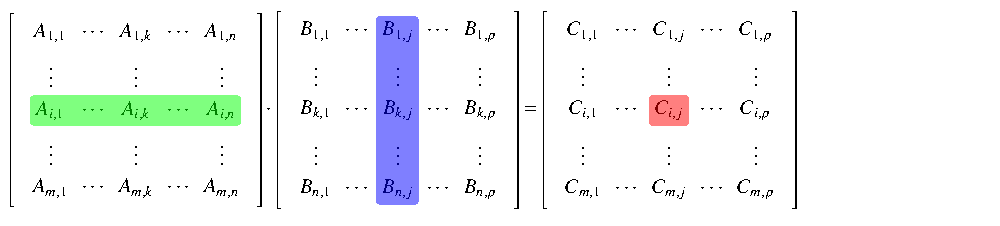
\includegraphics[]{papers/multiplikation/images/mm_visualisation}
	\caption{Grafische illustration der Matrizenmultiplikation}
	\label{multiplikation:fig:mm_viz}
\end{figure}
